\subsection{Runge's phenomenon}
A natural way to approximate a given function on any interval $[a,b]$ is to use an $n$-degree polynomial $p_n(x)$ by $n+1$ equispaced  points, namely
$$
x_i=a+{b-a\over n},\quad i=0,1,2,\cdots,n.
$$
By Weierstrass' theorem, we expect a more accurate reconstruction of $f(x)$ by using more points. But this is not always true as shown in the following example. 
%Consider the case where one desires to interpolate through $n+1$ equispaced points of a function $f(x)$ using the n-degree polynomial $p_n(x)$ that passes through those points. Naturally, one might expect from Weierstrass' theorem that using more points would lead to a more accurate reconstruction of $f(x)$. However, this particular set of polynomial functions $p_n(x)$ is not guaranteed to have the property of uniform convergence; the theorem only states that a set of polynomial functions exists, without providing a general method of finding one.

Consider the Runge function (a scaled version of the Witch of Agnesi)
$$ 
f(x)=\frac{1}{1+25x^{2}}.
$$
Runge found that if this function is interpolated at equidistant points $x_i$ between $-1$ and $1$ such that:
$$
x_{i}={\frac{2i}{n}}-1,\quad i\in \left\{0,1,\dots ,n\right\}
$$
with a polynomial $p_n(x)$ of degree $\leq n$, the resulting interpolation oscillates toward the ends of the interval, i.e. close to $-1$ and $1$. It can even be proven that the interpolation error increases (without bound) when the degree of the polynomial is increased:

$$\lim_{{n\rightarrow \infty }}\left(\max_{{-1\leq x\leq 1}}|f(x)-p_{n}(x)|\right)=+\infty.$$
This shows that high-degree polynomial interpolation at equidistant points can be troublesome.

\begin{figure}
	\begin{center}
		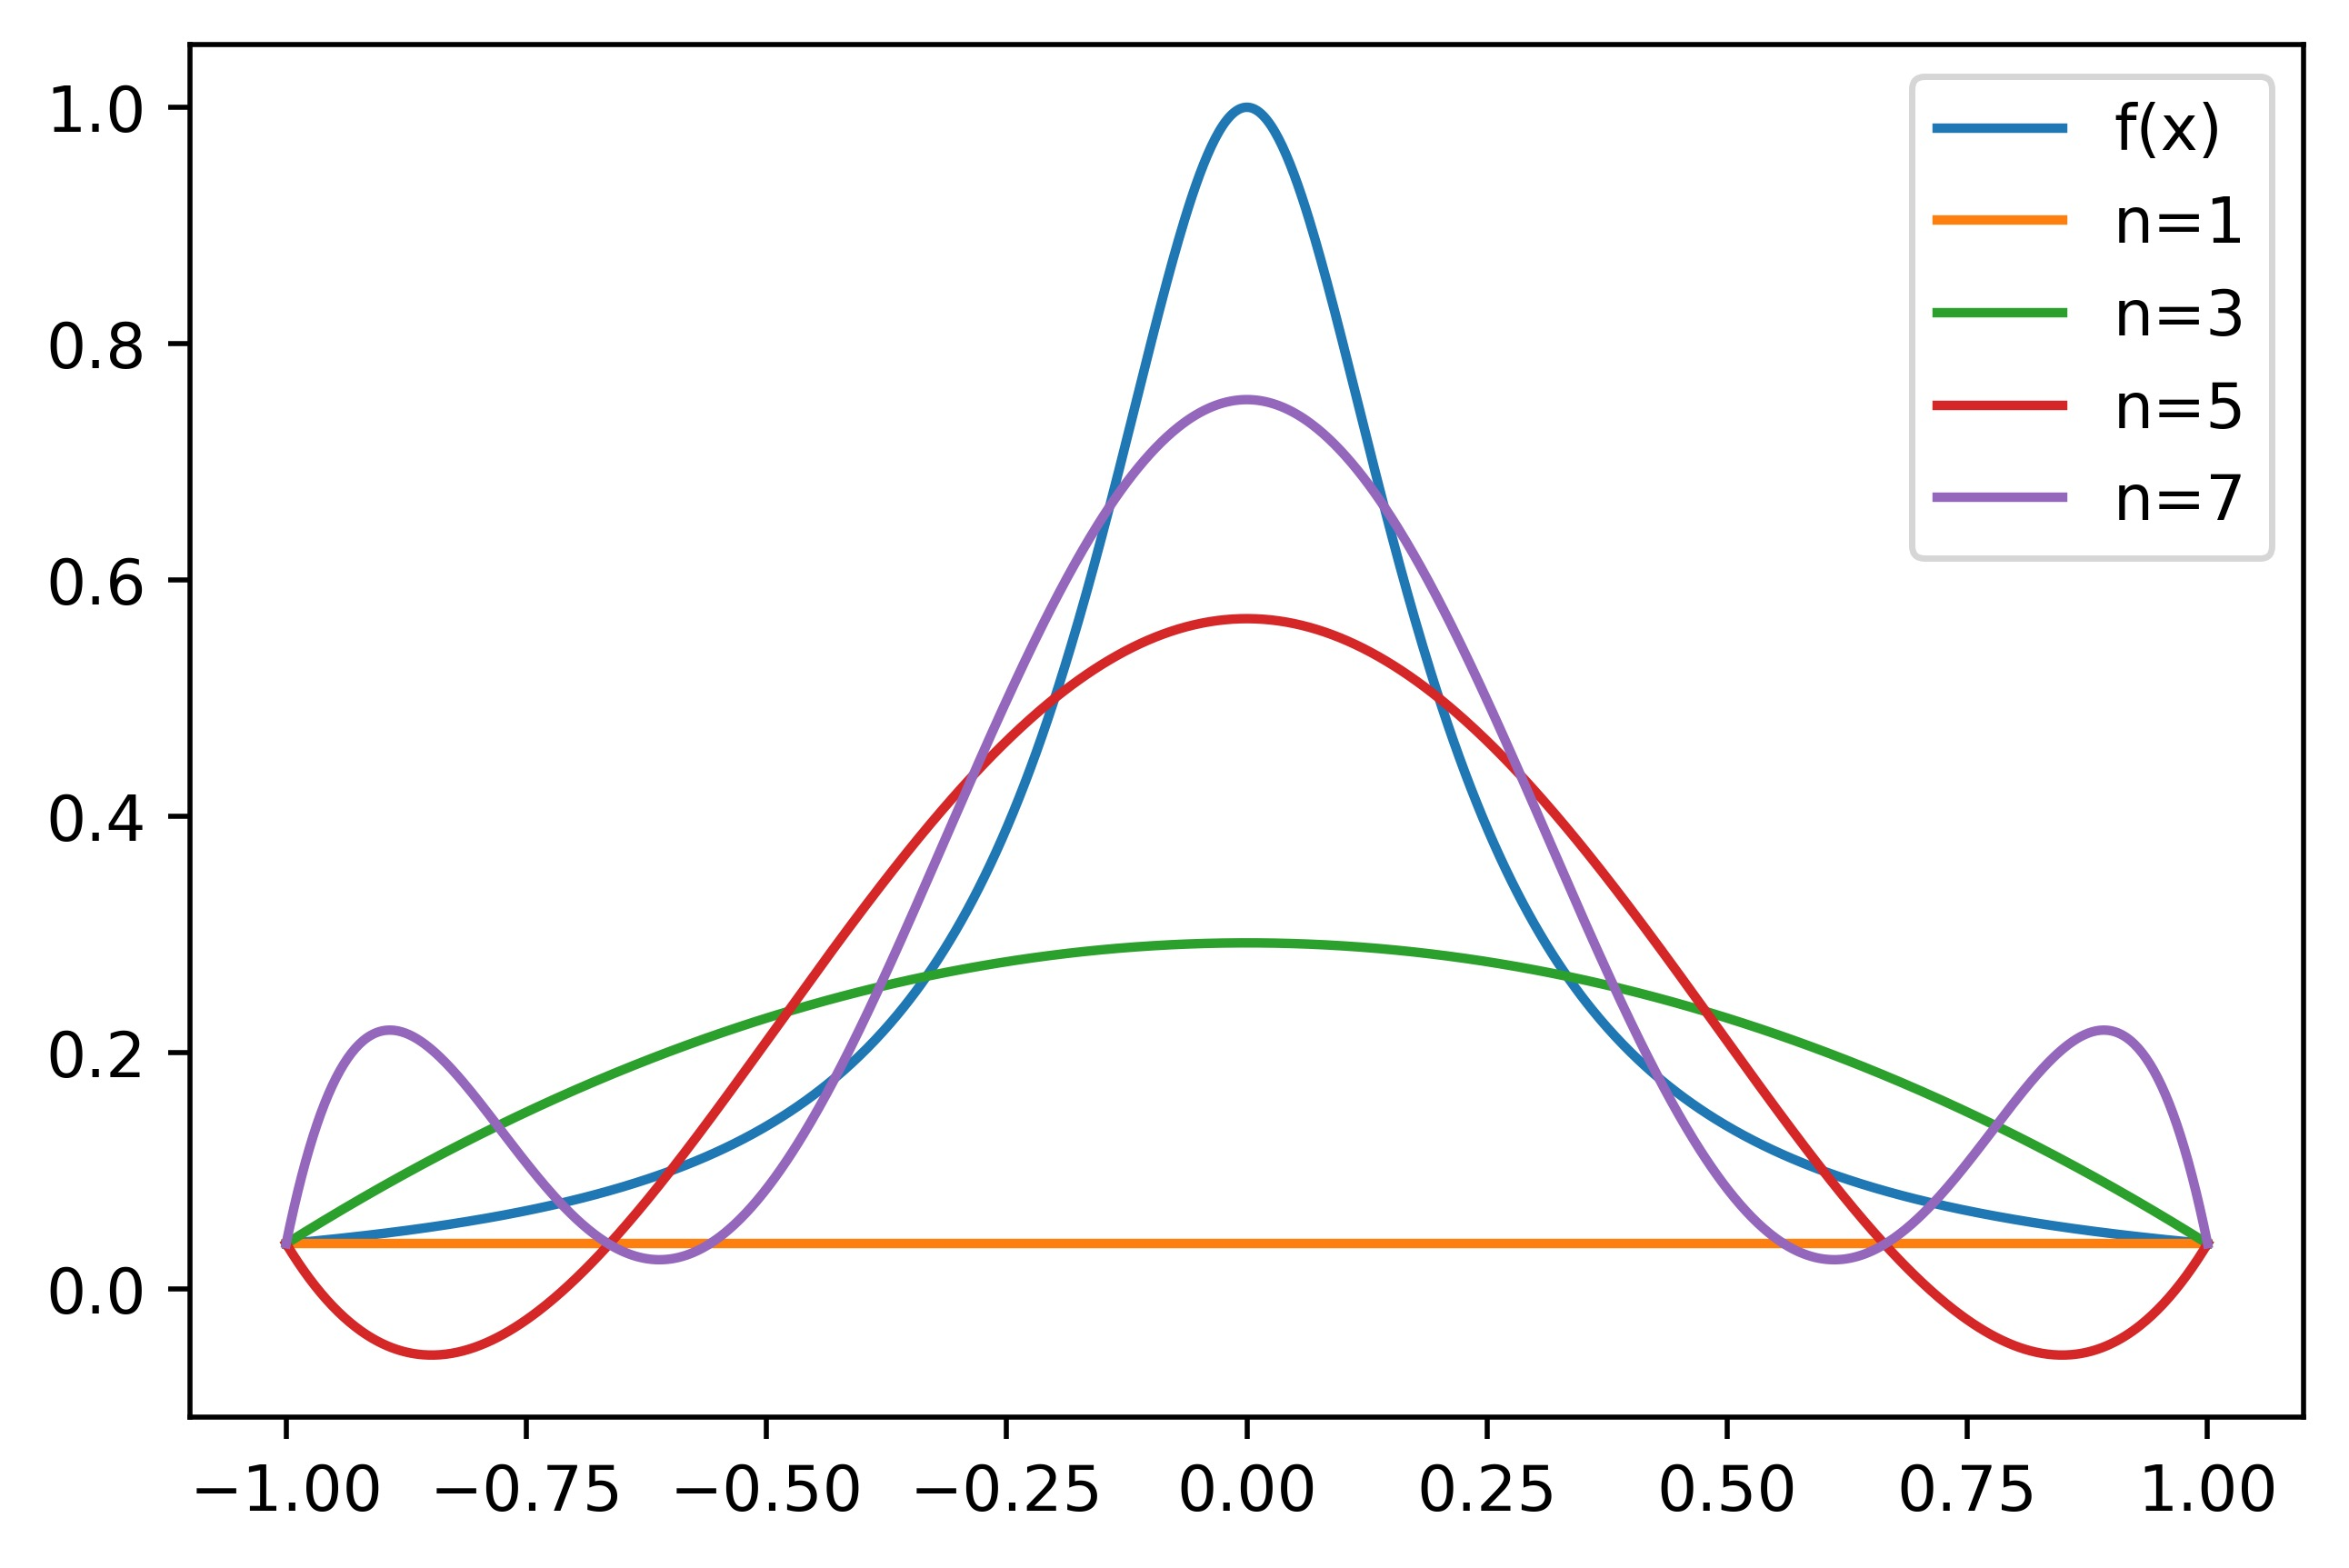
\includegraphics[scale=0.1]{6DL/pic/Runge.jpeg}
		\caption{Runge's phenomenon: Runge function $f(x)=\frac{1}{1+25x^{2}}$ and its polynomial interpolation $p_n(x)$.}
	\end{center}
\end{figure}

The experiment shows that  the polynomials $p_n(x)$ produced in this manner may in fact diverge away from $f(x)$ as $n$ increases. This typically occurs in an oscillating pattern that magnifies near the ends of the interpolation points. This phenomenon is attributed to Runge.

Thus, this particular set of polynomial functions $p_n(x)$ is not guaranteed to have the property of uniform convergence. In other words, Weierstrass' theorem guarantees the existence of the polynomial functions, but how to find such polynomials is not provided.
